%%%%%%%%%%%%%%%%%%%% author.tex %%%%%%%%%%%%%%%%%%%%%%%%%%%%%%%%%%%
%
% sample root file for your "contribution" to a proceedings volume
%
% Use this file as a template for your own input.
%
%%%%%%%%%%%%%%%% Springer %%%%%%%%%%%%%%%%%%%%%%%%%%%%%%%%%%
% to be used for MCQMC 2024
%%%%%%%%%%%%%%%%%%%%%%%%%%%%%%%%%%%%%%%%%%%%%%%%%%%%%%%%%%%%


\documentclass{svproc}
%
% RECOMMENDED %%%%%%%%%%%%%%%%%%%%%%%%%%%%%%%%%%%%%%%%%%%%%%%%%%%
%

% to typeset URLs, URIs, and DOIs
\usepackage{url}
\def\UrlFont{\rmfamily}

%%%%%%%added CL
\usepackage{hyperref}
\usepackage{type1cm}        % activate if the above 3 fonts are
% not available on your system
%
\usepackage{makeidx}         % allows index generation
\usepackage{graphicx}        % standard LaTeX graphics tool
                             % when including figure files
%%% if you are including figures and images, you are encouraged to put them in sub-directory(ies)
%%% whose path(s) can be provided using the following command
%%% \graphicspath{{<path 1>}{<path 2>}}
%%% for example if your sub-directory is called MyFigures then you would use the command
%%% \graphicspath{{MyFigures/}}


\usepackage{multicol}        % used for the two-column index
\usepackage[bottom]{footmisc}% places footnotes at page bottom


\usepackage{newtxtext}       %
\usepackage[varvw]{newtxmath}       % selects Times Roman as basic font

% see the list of further useful packages
% in the Reference Guide

%\makeindex             % used for the subject index
% please use the style svind.ist with
% your makeindex program

%%%%%%%%%%%%%%%%%%%%%%%%%%%%%%%%%%%%%%%%%%%%%%%%%%%%%%%%%%%%%%%%%%%%%%%%%%%%%%%%%%%%%%%%%

% Additional packages
\usepackage{bm}% for bold math symbols
\usepackage{siunitx}% for table alignments

% Additional environment
% \usepackage{amsmath}
% \newtheorem{algorithm}{\upshape Algorithm}[1][]

\newcounter{algorithm}%[section]
\newenvironment{algorithm}[1][]{\refstepcounter{algorithm}\par\medskip
  \noindent\textbf{Algorithm~\thealgorithm\mbox{ }#1}}{\medskip}


%%  This file will be included when we compile the final book. You can
%%  make use of the commonly used packages and commonly defined macros
%%  from here.
%%
%%  PLEASE DO NOT CHANGE THIS FILE.
%%  PLEASE DO NOT REDFINE ANY OF THE MACROS.
%%
%%  For convenience you may wish to define your own macros in your main
%%  tex file while preparing the manuscript. However, before submitting
%%  your final file for the accepted manuscript, we will ask you to replace
%%  your macros with the full commands.
%%

%% OCTOBER 2021 VERSION

% We add the following commonly used macros:

% vectors as boldsymbols:
\newcommand{\bsa}{{\boldsymbol{a}}}
\newcommand{\bsb}{{\boldsymbol{b}}}
\newcommand{\bsc}{{\boldsymbol{c}}}
\newcommand{\bsd}{{\boldsymbol{d}}}
\newcommand{\bse}{{\boldsymbol{e}}}
\newcommand{\bsf}{{\boldsymbol{f}}}
\newcommand{\bsg}{{\boldsymbol{g}}}
\newcommand{\bsh}{{\boldsymbol{h}}}
\newcommand{\bsi}{{\boldsymbol{i}}}
\newcommand{\bsj}{{\boldsymbol{j}}}
\newcommand{\bsk}{{\boldsymbol{k}}}
\newcommand{\bsl}{{\boldsymbol{l}}}
\newcommand{\bsm}{{\boldsymbol{m}}}
\newcommand{\bsn}{{\boldsymbol{n}}}
\newcommand{\bso}{{\boldsymbol{o}}}
\newcommand{\bsp}{{\boldsymbol{p}}}
\newcommand{\bsq}{{\boldsymbol{q}}}
\newcommand{\bsr}{{\boldsymbol{r}}}
\newcommand{\bss}{{\boldsymbol{s}}}
\newcommand{\bst}{{\boldsymbol{t}}}
\newcommand{\bsu}{{\boldsymbol{u}}}
\newcommand{\bsv}{{\boldsymbol{v}}}
\newcommand{\bsw}{{\boldsymbol{w}}}
\newcommand{\bsx}{{\boldsymbol{x}}}
\newcommand{\bsy}{{\boldsymbol{y}}}
\newcommand{\bsz}{{\boldsymbol{z}}}
\newcommand{\bsA}{{\boldsymbol{A}}}
\newcommand{\bsB}{{\boldsymbol{B}}}
\newcommand{\bsC}{{\boldsymbol{C}}}
\newcommand{\bsD}{{\boldsymbol{D}}}
\newcommand{\bsE}{{\boldsymbol{E}}}
\newcommand{\bsF}{{\boldsymbol{F}}}
\newcommand{\bsG}{{\boldsymbol{G}}}
\newcommand{\bsH}{{\boldsymbol{H}}}
\newcommand{\bsI}{{\boldsymbol{I}}}
\newcommand{\bsJ}{{\boldsymbol{J}}}
\newcommand{\bsK}{{\boldsymbol{K}}}
\newcommand{\bsL}{{\boldsymbol{L}}}
\newcommand{\bsM}{{\boldsymbol{M}}}
\newcommand{\bsN}{{\boldsymbol{N}}}
\newcommand{\bsO}{{\boldsymbol{O}}}
\newcommand{\bsP}{{\boldsymbol{P}}}
\newcommand{\bsQ}{{\boldsymbol{Q}}}
\newcommand{\bsR}{{\boldsymbol{R}}}
\newcommand{\bsS}{{\boldsymbol{S}}}
\newcommand{\bsT}{{\boldsymbol{T}}}
\newcommand{\bsU}{{\boldsymbol{U}}}
\newcommand{\bsV}{{\boldsymbol{V}}}
\newcommand{\bsW}{{\boldsymbol{W}}}
\newcommand{\bsX}{{\boldsymbol{X}}}
\newcommand{\bsY}{{\boldsymbol{Y}}}
\newcommand{\bsZ}{{\boldsymbol{Z}}}
% other commonly used boldsymbols:
\newcommand{\bsell}{{\boldsymbol{\ell}}}
\newcommand{\bszero}{{\boldsymbol{0}}} % vector of zeros
\newcommand{\bsone}{{\boldsymbol{1}}}  % vector of ones
% boldsymbol greeks:
\newcommand{\bsalpha}{{\boldsymbol{\alpha}}}
\newcommand{\bsbeta}{{\boldsymbol{\beta}}}
\newcommand{\bsgamma}{{\boldsymbol{\gamma}}}
\newcommand{\bsdelta}{{\boldsymbol{\delta}}}
\newcommand{\bsepsilon}{{\boldsymbol{\epsilon}}}
\newcommand{\bsvarepsilon}{{\boldsymbol{\varepsilon}}}
\newcommand{\bszeta}{{\boldsymbol{\zeta}}}
\newcommand{\bseta}{{\boldsymbol{\eta}}}
\newcommand{\bstheta}{{\boldsymbol{\theta}}}
\newcommand{\bsvartheta}{{\boldsymbol{\vartheta}}}
\newcommand{\bskappa}{{\boldsymbol{\kappa}}}
\newcommand{\bslambda}{{\boldsymbol{\lambda}}}
\newcommand{\bsmu}{{\boldsymbol{\mu}}}
\newcommand{\bsnu}{{\boldsymbol{\nu}}}
\newcommand{\bsxi}{{\boldsymbol{\xi}}}
\newcommand{\bspi}{{\boldsymbol{\pi}}}
\newcommand{\bsvarpi}{{\boldsymbol{\varpi}}}
\newcommand{\bsrho}{{\boldsymbol{\rho}}}
\newcommand{\bsvarrho}{{\boldsymbol{\varrho}}}
\newcommand{\bssigma}{{\boldsymbol{\sigma}}}
\newcommand{\bsvarsigma}{{\boldsymbol{\varsigma}}}
\newcommand{\bstau}{{\boldsymbol{\tau}}}
\newcommand{\bsupsilon}{{\boldsymbol{\upsilon}}}
\newcommand{\bsphi}{{\boldsymbol{\phi}}}
\newcommand{\bsvarphi}{{\boldsymbol{\varphi}}}
\newcommand{\bschi}{{\boldsymbol{\chi}}}
\newcommand{\bspsi}{{\boldsymbol{\psi}}}
\newcommand{\bsomega}{{\boldsymbol{\omega}}}
\newcommand{\bsGamma}{{\boldsymbol{\Gamma}}}
\newcommand{\bsDelta}{{\boldsymbol{\Delta}}}
\newcommand{\bsTheta}{{\boldsymbol{\Theta}}}
\newcommand{\bsLambda}{{\boldsymbol{\Lambda}}}
\newcommand{\bsXi}{{\boldsymbol{\Xi}}}
\newcommand{\bsPi}{{\boldsymbol{\Pi}}}
\newcommand{\bsSigma}{{\boldsymbol{\Sigma}}}
\newcommand{\bsUpsilon}{{\boldsymbol{\Upsilon}}}
\newcommand{\bsPhi}{{\boldsymbol{\Phi}}}
\newcommand{\bsPsi}{{\boldsymbol{\Psi}}}
\newcommand{\bsOmega}{{\boldsymbol{\Omega}}}

% Roman fonts:
\newcommand{\rma}{{\mathrm{a}}}
\newcommand{\rmb}{{\mathrm{b}}}
\newcommand{\rmc}{{\mathrm{c}}}
\newcommand{\rmd}{{\mathrm{d}}}
\newcommand{\rme}{{\mathrm{e}}}
\newcommand{\rmf}{{\mathrm{f}}}
\newcommand{\rmg}{{\mathrm{g}}}
\newcommand{\rmh}{{\mathrm{h}}}
\newcommand{\rmi}{{\mathrm{i}}}
\newcommand{\rmj}{{\mathrm{j}}}
\newcommand{\rmk}{{\mathrm{k}}}
\newcommand{\rml}{{\mathrm{l}}}
\newcommand{\rmm}{{\mathrm{m}}}
\newcommand{\rmn}{{\mathrm{n}}}
\newcommand{\rmo}{{\mathrm{o}}}
\newcommand{\rmp}{{\mathrm{p}}}
\newcommand{\rmq}{{\mathrm{q}}}
\newcommand{\rmr}{{\mathrm{r}}}
\newcommand{\rms}{{\mathrm{s}}}
\newcommand{\rmt}{{\mathrm{t}}}
\newcommand{\rmu}{{\mathrm{u}}}
\newcommand{\rmv}{{\mathrm{v}}}
\newcommand{\rmw}{{\mathrm{w}}}
\newcommand{\rmx}{{\mathrm{x}}}
\newcommand{\rmy}{{\mathrm{y}}}
\newcommand{\rmz}{{\mathrm{z}}}
\newcommand{\rmA}{{\mathrm{A}}}
\newcommand{\rmB}{{\mathrm{B}}}
\newcommand{\rmC}{{\mathrm{C}}}
\newcommand{\rmD}{{\mathrm{D}}}
\newcommand{\rmE}{{\mathrm{E}}}
\newcommand{\rmF}{{\mathrm{F}}}
\newcommand{\rmG}{{\mathrm{G}}}
\newcommand{\rmH}{{\mathrm{H}}}
\newcommand{\rmI}{{\mathrm{I}}}
\newcommand{\rmJ}{{\mathrm{J}}}
\newcommand{\rmK}{{\mathrm{K}}}
\newcommand{\rmL}{{\mathrm{L}}}
\newcommand{\rmM}{{\mathrm{M}}}
\newcommand{\rmN}{{\mathrm{N}}}
\newcommand{\rmO}{{\mathrm{O}}}
\newcommand{\rmP}{{\mathrm{P}}}
\newcommand{\rmQ}{{\mathrm{Q}}}
\newcommand{\rmR}{{\mathrm{R}}}
\newcommand{\rmS}{{\mathrm{S}}}
\newcommand{\rmT}{{\mathrm{T}}}
\newcommand{\rmU}{{\mathrm{U}}}
\newcommand{\rmV}{{\mathrm{V}}}
\newcommand{\rmW}{{\mathrm{W}}}
\newcommand{\rmX}{{\mathrm{X}}}
\newcommand{\rmY}{{\mathrm{Y}}}
\newcommand{\rmZ}{{\mathrm{Z}}}
% also commonly defined
\newcommand{\rd}{{\mathrm{d}}}
\newcommand{\ri}{{\mathrm{i}}}

% blackboards:
\newcommand{\bbA}{{\mathbb{A}}}
\newcommand{\bbB}{{\mathbb{B}}}
\newcommand{\bbC}{{\mathbb{C}}}
\newcommand{\bbD}{{\mathbb{D}}}
\newcommand{\bbE}{{\mathbb{E}}}
\newcommand{\bbF}{{\mathbb{F}}}
\newcommand{\bbG}{{\mathbb{G}}}
\newcommand{\bbH}{{\mathbb{H}}}
\newcommand{\bbI}{{\mathbb{I}}}
\newcommand{\bbJ}{{\mathbb{J}}}
\newcommand{\bbK}{{\mathbb{K}}}
\newcommand{\bbL}{{\mathbb{L}}}
\newcommand{\bbM}{{\mathbb{M}}}
\newcommand{\bbN}{{\mathbb{N}}}
\newcommand{\bbO}{{\mathbb{O}}}
\newcommand{\bbP}{{\mathbb{P}}}
\newcommand{\bbQ}{{\mathbb{Q}}}
\newcommand{\bbR}{{\mathbb{R}}}
\newcommand{\bbS}{{\mathbb{S}}}
\newcommand{\bbT}{{\mathbb{T}}}
\newcommand{\bbU}{{\mathbb{U}}}
\newcommand{\bbV}{{\mathbb{V}}}
\newcommand{\bbW}{{\mathbb{W}}}
\newcommand{\bbX}{{\mathbb{X}}}
\newcommand{\bbY}{{\mathbb{Y}}}
\newcommand{\bbZ}{{\mathbb{Z}}}
% commonly used shortcuts:
\newcommand{\C}{{\mathbb{C}}} % complex numbers
\newcommand{\F}{{\mathbb{F}}} % field, finite field
\newcommand{\N}{{\mathbb{N}}} % natural numbers {1, 2, ...}
\newcommand{\Q}{{\mathbb{Q}}} % rationals
\newcommand{\R}{{\mathbb{R}}} % reals
\newcommand{\Z}{{\mathbb{Z}}} % integers
% more commonly used shortcuts:
\newcommand{\CC}{{\mathbb{C}}} % complex numbers
\newcommand{\FF}{{\mathbb{F}}} % field, finite field
\newcommand{\NN}{{\mathbb{N}}} % natural numbers {1, 2, ...}
\newcommand{\QQ}{{\mathbb{Q}}} % rationals
\newcommand{\RR}{{\mathbb{R}}} % reals
\newcommand{\ZZ}{{\mathbb{Z}}} % integers
% more commonly used shortcuts:
\newcommand{\EE}{{\mathbb{E}}}
\newcommand{\PP}{{\mathbb{P}}}
\newcommand{\TT}{{\mathbb{T}}}
\newcommand{\VV}{{\mathbb{V}}}
% and even more commonly used shortcuts:
\newcommand{\Complex}{{\mathbb{C}}}
\newcommand{\Integer}{{\mathbb{Z}}}
\newcommand{\Natural}{{\mathbb{N}}}
\newcommand{\Rational}{{\mathbb{Q}}}
\newcommand{\Real}{{\mathbb{R}}}
% indicator boldface 1:
\DeclareSymbolFont{bbold}{U}{bbold}{m}{n}
\DeclareSymbolFontAlphabet{\mathbbold}{bbold}
\newcommand{\ind}{{\mathbbold{1}}}
\newcommand{\bbone}{{\mathbbold{1}}}


% calligraphic letters:
\newcommand{\cala}{{\mathcal{a}}}
\newcommand{\calb}{{\mathcal{b}}}
\newcommand{\calc}{{\mathcal{c}}}
\newcommand{\cald}{{\mathcal{d}}}
\newcommand{\cale}{{\mathcal{e}}}
\newcommand{\calf}{{\mathcal{f}}}
\newcommand{\calg}{{\mathcal{g}}}
\newcommand{\calh}{{\mathcal{h}}}
\newcommand{\cali}{{\mathcal{i}}}
\newcommand{\calj}{{\mathcal{j}}}
\newcommand{\calk}{{\mathcal{k}}}
\newcommand{\call}{{\mathcal{l}}}
\newcommand{\calm}{{\mathcal{m}}}
\newcommand{\caln}{{\mathcal{n}}}
\newcommand{\calo}{{\mathcal{o}}}
\newcommand{\calp}{{\mathcal{p}}}
\newcommand{\calq}{{\mathcal{q}}}
\newcommand{\calr}{{\mathcal{r}}}
\newcommand{\cals}{{\mathcal{s}}}
\newcommand{\calt}{{\mathcal{t}}}
\newcommand{\calu}{{\mathcal{u}}}
\newcommand{\calv}{{\mathcal{v}}}
\newcommand{\calw}{{\mathcal{w}}}
\newcommand{\calx}{{\mathcal{x}}}
\newcommand{\caly}{{\mathcal{y}}}
\newcommand{\calz}{{\mathcal{z}}}
\newcommand{\calA}{{\mathcal{A}}}
\newcommand{\calB}{{\mathcal{B}}}
\newcommand{\calC}{{\mathcal{C}}}
\newcommand{\calD}{{\mathcal{D}}}
\newcommand{\calE}{{\mathcal{E}}}
\newcommand{\calF}{{\mathcal{F}}}
\newcommand{\calG}{{\mathcal{G}}}
\newcommand{\calH}{{\mathcal{H}}}
\newcommand{\calI}{{\mathcal{I}}}
\newcommand{\calJ}{{\mathcal{J}}}
\newcommand{\calK}{{\mathcal{K}}}
\newcommand{\calL}{{\mathcal{L}}}
\newcommand{\calM}{{\mathcal{M}}}
\newcommand{\calN}{{\mathcal{N}}}
\newcommand{\calO}{{\mathcal{O}}}
\newcommand{\calP}{{\mathcal{P}}}
\newcommand{\calQ}{{\mathcal{Q}}}
\newcommand{\calR}{{\mathcal{R}}}
\newcommand{\calS}{{\mathcal{S}}}
\newcommand{\calT}{{\mathcal{T}}}
\newcommand{\calU}{{\mathcal{U}}}
\newcommand{\calV}{{\mathcal{V}}}
\newcommand{\calW}{{\mathcal{W}}}
\newcommand{\calX}{{\mathcal{X}}}
\newcommand{\calY}{{\mathcal{Y}}}
\newcommand{\calZ}{{\mathcal{Z}}}

% Euler fraks:
\newcommand{\fraka}{{\mathfrak{a}}}
\newcommand{\frakb}{{\mathfrak{b}}}
\newcommand{\frakc}{{\mathfrak{c}}}
\newcommand{\frakd}{{\mathfrak{d}}}
\newcommand{\frake}{{\mathfrak{e}}}
\newcommand{\frakf}{{\mathfrak{f}}}
\newcommand{\frakg}{{\mathfrak{g}}}
\newcommand{\frakh}{{\mathfrak{h}}}
\newcommand{\fraki}{{\mathfrak{i}}}
\newcommand{\frakj}{{\mathfrak{j}}}
\newcommand{\frakk}{{\mathfrak{k}}}
\newcommand{\frakl}{{\mathfrak{l}}}
\newcommand{\frakm}{{\mathfrak{m}}}
\newcommand{\frakn}{{\mathfrak{n}}}
\newcommand{\frako}{{\mathfrak{o}}}
\newcommand{\frakp}{{\mathfrak{p}}}
\newcommand{\frakq}{{\mathfrak{q}}}
\newcommand{\frakr}{{\mathfrak{r}}}
\newcommand{\fraks}{{\mathfrak{s}}}
\newcommand{\frakt}{{\mathfrak{t}}}
\newcommand{\fraku}{{\mathfrak{u}}}
\newcommand{\frakv}{{\mathfrak{v}}}
\newcommand{\frakw}{{\mathfrak{w}}}
\newcommand{\frakx}{{\mathfrak{x}}}
\newcommand{\fraky}{{\mathfrak{y}}}
\newcommand{\frakz}{{\mathfrak{z}}}
\newcommand{\frakA}{{\mathfrak{A}}}
\newcommand{\frakB}{{\mathfrak{B}}}
\newcommand{\frakC}{{\mathfrak{C}}}
\newcommand{\frakD}{{\mathfrak{D}}}
\newcommand{\frakE}{{\mathfrak{E}}}
\newcommand{\frakF}{{\mathfrak{F}}}
\newcommand{\frakG}{{\mathfrak{G}}}
\newcommand{\frakH}{{\mathfrak{H}}}
\newcommand{\frakI}{{\mathfrak{I}}}
\newcommand{\frakJ}{{\mathfrak{J}}}
\newcommand{\frakK}{{\mathfrak{K}}}
\newcommand{\frakL}{{\mathfrak{L}}}
\newcommand{\frakM}{{\mathfrak{M}}}
\newcommand{\frakN}{{\mathfrak{N}}}
\newcommand{\frakO}{{\mathfrak{O}}}
\newcommand{\frakP}{{\mathfrak{P}}}
\newcommand{\frakQ}{{\mathfrak{Q}}}
\newcommand{\frakR}{{\mathfrak{R}}}
\newcommand{\frakS}{{\mathfrak{S}}}
\newcommand{\frakT}{{\mathfrak{T}}}
\newcommand{\frakU}{{\mathfrak{U}}}
\newcommand{\frakV}{{\mathfrak{V}}}
\newcommand{\frakW}{{\mathfrak{W}}}
\newcommand{\frakX}{{\mathfrak{X}}}
\newcommand{\frakY}{{\mathfrak{Y}}}
\newcommand{\frakZ}{{\mathfrak{Z}}}
% sets as Euler fraks:
\newcommand{\seta}{{\mathfrak{a}}}
\newcommand{\setb}{{\mathfrak{b}}}
\newcommand{\setc}{{\mathfrak{c}}}
\newcommand{\setd}{{\mathfrak{d}}}
\newcommand{\sete}{{\mathfrak{e}}}
\newcommand{\setf}{{\mathfrak{f}}}
\newcommand{\setg}{{\mathfrak{g}}}
\newcommand{\seth}{{\mathfrak{h}}}
\newcommand{\seti}{{\mathfrak{i}}}
\newcommand{\setj}{{\mathfrak{j}}}
\newcommand{\setk}{{\mathfrak{k}}}
\newcommand{\setl}{{\mathfrak{l}}}
\newcommand{\setm}{{\mathfrak{m}}}
\newcommand{\setn}{{\mathfrak{n}}}
\newcommand{\seto}{{\mathfrak{o}}}
\newcommand{\setp}{{\mathfrak{p}}}
\newcommand{\setq}{{\mathfrak{q}}}
\newcommand{\setr}{{\mathfrak{r}}}
\newcommand{\sets}{{\mathfrak{s}}}
\newcommand{\sett}{{\mathfrak{t}}}
\newcommand{\setu}{{\mathfrak{u}}}
\newcommand{\setv}{{\mathfrak{v}}}
\newcommand{\setw}{{\mathfrak{w}}}
\newcommand{\setx}{{\mathfrak{x}}}
\newcommand{\sety}{{\mathfrak{y}}}
\newcommand{\setz}{{\mathfrak{z}}}
\newcommand{\setA}{{\mathfrak{A}}}
\newcommand{\setB}{{\mathfrak{B}}}
\newcommand{\setC}{{\mathfrak{C}}}
\newcommand{\setD}{{\mathfrak{D}}}
\newcommand{\setE}{{\mathfrak{E}}}
\newcommand{\setF}{{\mathfrak{F}}}
\newcommand{\setG}{{\mathfrak{G}}}
\newcommand{\setH}{{\mathfrak{H}}}
\newcommand{\setI}{{\mathfrak{I}}}
\newcommand{\setJ}{{\mathfrak{J}}}
\newcommand{\setK}{{\mathfrak{K}}}
\newcommand{\setL}{{\mathfrak{L}}}
\newcommand{\setM}{{\mathfrak{M}}}
\newcommand{\setN}{{\mathfrak{N}}}
\newcommand{\setO}{{\mathfrak{O}}}
\newcommand{\setP}{{\mathfrak{P}}}
\newcommand{\setQ}{{\mathfrak{Q}}}
\newcommand{\setR}{{\mathfrak{R}}}
\newcommand{\setS}{{\mathfrak{S}}}
\newcommand{\setT}{{\mathfrak{T}}}
\newcommand{\setU}{{\mathfrak{U}}}
\newcommand{\setV}{{\mathfrak{V}}}
\newcommand{\setW}{{\mathfrak{W}}}
\newcommand{\setX}{{\mathfrak{X}}}
\newcommand{\setY}{{\mathfrak{Y}}}
\newcommand{\setZ}{{\mathfrak{Z}}}

% other commonly defined commands:
\newcommand{\wal}{{\rm wal}}
\newcommand{\floor}[1]{\left\lfloor #1 \right\rfloor} % floor
\newcommand{\ceil}[1]{\left\lceil #1 \right\rceil}    % ceil
\DeclareMathOperator{\cov}{Cov}
\DeclareMathOperator{\var}{Var}
\providecommand{\argmin}{\operatorname*{argmin}}
\providecommand{\argmax}{\operatorname*{argmax}}
%%%% end added CL


%%Fred's temporary macros
\newcommand{\figpath}{Figures}
\usepackage{xspace}

%%End of Fred's temporary macros


\begin{document}


\mainmatter              % start of a contribution
%
\title{Quasi-Monte Carlo Methods:  What, Why, and How?}
%
\titlerunning{Quasi-Monte Carlo Methods}  % abbreviated title (for running head)
%                                     also used for the TOC unless
%                                     \toctitle is used
%
\author{Fred J. Hickernell\inst{1} \and Aleksei G. Sorokin\inst{2}}
%
\authorrunning{Hickernell and Sorokin} % abbreviated author list (for running head)
%
%%%% list of authors for the TOC (use if author list has to be modified)
\tocauthor{Fred J. Hickernell, Aleksei G. Sorokin}
%
\institute{Departmet of Applied Mathematics, Illinois Institute of Technology, Chicago, IL, 60616, USA\\
\email{hickernell@iit.edu}, \
\texttt{http://www.iit.edu/~hickernell}
\and
Departmet of Applied Mathematics, Illinois Institute of Technology, Chicago, IL, 60616, USA\\
\email{asorokin@hawk.iit.edu}}

\maketitle              % typeset the title of the contribution

\begin{abstract}
Many problems in  quantitative finance, uncertainty quantification, and other areas have answers of the form $\mu := \mathbb{E}(Y)$, where instances of $Y:=f(\boldsymbol{X})$ may be generated by numerical simulation. The population mean, $\mu$, can be approximated by the sample mean, $\hat{\mu}_n := n^{-1} \sum_{i=0}^{n-1} f(\bsx_i)$ for a well chosen sequence of nodes, $\{\bsx_0, \bsx_1, \ldots\}$.  Computing $\mu$ is equivalent to computing a $d$-dimensional integral.

Quasi-Monte Carlo methods replace independent and identically distributed  sequences of random vector nodes, $\{\boldsymbol{X}_i \}$, by low discrepancy sequences.  This accelerates the convergence of $\hat{\mu}_n$ to $\mu$ as $n \to \infty$.

This tutorial describes  low discrepancy sequences  and their quality measures.  We demonstrate the performance gains possible with quasi-Monte Carlo methods.  Moreover, we describe how to formulate problems to realize the most increase in performance using quasi-Monte Carlo methods.  We also briefly describe the use of quasi-Monte Carlo methods for problems beyond computing the mean, $\mu$.

\keywords{}
\end{abstract}
%
\section{Introduction} \label{sec:intro}
There are may settings where key underlying quantities that affect the outcome are unknown, e.g.,
\begin{itemize}
	\item Future market forces, which affect financial risk,
	\item The porosity of rock, which affect the extraction of oil or gas, or
	\item Elemetary particle interactions in a high energy physics experiment, which affect what is observed by detectors.
\end{itemize}
In such situations, the unknown inputs are often modeled using random variables or stochastic processes.  Computations are performed by generating a multidude of possible scenarios informed by the assumed probability distribution of the input. These are used to estimate the mean, quantiles, and/or probability distribution of the outcome.  This is the essence of the Monte Carlo (MC) method.

In mathematical terms, the outcome is $Y := f(\bsX)$, where $\bsX$ is a vector random variable of inputs determining the outcome.  The values of $f$ can be computed by an algorithm, whose complexity may be such that $f$ can be considered a ``black box''.  The scenarios are $\bsx_0, \bsx_1, \ldots$, which give rise to outcomes $y_0 = f(\bsx_0), y_1 = f(\bsx_1), \ldots$.  The $y_i$ form the basis for approximating $\bbE(Y)$ and other quantities of interest. These scenarios are also commonly called instances of $\bsX$ or nodes.  We use these terms interchangeably.

Simple or independent and identically distributed (IID)  Monte Carlo chooses the sequence of nodes $\{\bsx_0, \bsx_1, \ldots\}$ to be IID.  Quasi-Monte Carlo (qMC) methods choose the nodes to be \emph{not} IID, but with an empirical distribution that approximates well the true probability distribution of $\bsX$.  The difference between these two distributions is called a \emph{discrepancy}, and the node sequences used in qMC are called low discrepancy (LD) sequences.

This tutorial describes what qMC is, why we would want to use qMC, and how qMC can be implemented well.  The next session provides an illustrative example of the advantages of qMC.  This is followed by a description of how LD sequences are constructed and various measures of discrepancy.  We then explain how randomization can improve qMC, how to decide what sample size, $n$, is sufficient, and how to rewrite the problem of interest in a qMC-friendly way.


%
\section{An Illustration of Quasi-Monte Carlo} \label{sec:practice}

To illustrate the benefits of qMC, consider the example from Keister \cite[(13)]{Kei96}, motivated by computational physics:

\begin{equation}\label{eq:keisterA}
	\mu := \int_{\mathbb{R}^d} \cos(\lVert \bst \rVert) \exp(-\lVert \bst \rVert^2) \, \rmd \bst,
\end{equation}
where $\lVert \bst \rVert := \sqrt{t_1^2 + \cdots + t_d^2}$.  This integral may be evaluated numerically by re-writing it in spherical coordinates as
\begin{equation}\label{eq:keisterExact}
	\mu = \frac{2 \pi^{d/2}}{\Gamma(d/2)}\int_{0}^{\infty} \cos(r) \exp(-r^2) \, r^{d-1} \rmd r,
\end{equation}
where $2 \pi^{d/2}/\Gamma(d/2)$ is the surface area of the sphere in $d$ dimensions, and $\Gamma$ is the Gamma function.  This non-trivial test case with a true value that can be easily calculated allows us to compute the numerical errors of various cubature schemes.

The aim is to approximate $\mu$ by a sample mean,
\begin{equation} \label{eq:sample_mean}
	\hat{\mu}_n := \frac 1n \sum_{i=1}^n f(\bsx_i),
\end{equation}
but to do so requires some further preparation.  More on this preparation process is discussed in Section \ref{sec:reformulate}.

This integral, $\mu$, may be thought of as the expectation of $Y := g(\bsT) := \pi^{d/2} \cos(\lVert \bsT \rVert)$, where $T_1, \ldots, T_d$ are IID Gaussian random variables with zero mean and variance $1/2$, i.e., $\bsT :=(T_1, \ldots, T_d) \sim \calN(\bszero,\mathsf{I}/2)$:
\begin{equation}\label{eq:keisterB}
	\mu = \int_{\mathbb{R}^d} \underbrace{\pi^{d/2} \cos(\lVert \bst \rVert)}_{=:g(\bst)} \cdot \underbrace{\frac{\exp(-\lVert \bst \rVert^2)}{\pi^{d/2}}}_{\text{density of } \calN(\bszero,\mathsf{I}/2)} \, \rmd \bst = \bbE(Y) = \bbE[g(\bsT)].
\end{equation}

Since the LD sequences that underly qMC are defined to approximate the standard uniform distribution, we perform a variable transformation $\bst = \bigl (\Phi^{-1}(x_1), \ldots, \Phi^{-1}(x_d) \bigr )/\sqrt{2}$, where is $\Phi$ is the cumulative distribution function of the standard Gaussian random variable.  This reimagines the integral $\mu$ as the expectation of a function, $f$, of a standard uniform random variable:
\begin{multline}\label{eq:keisterC}
	\mu = \int_{[0,1]^d} \underbrace{\pi^{d/2} \cos\Bigl (\bigl \lVert \bigl( \Phi^{-1}(x_1), \ldots, \Phi^{-1}(x_d)\bigr) \bigr\rVert/\sqrt{2}  \Bigr)}_{=:f(\bsx)} \, \rmd \bsx \\
	= \bbE[Y]
	= \bbE[f(\bsX)], \qquad \bsX \sim \calU[0,1]^d.
\end{multline}

Consider the specific case of $d=6$ for which $\mu \approx -2.327303729298$.  We approximate $\mu$ by the sample mean defined in \eqref{eq:sample_mean} for three different kinds of nodes, $\{\bsx_i\}_{i=0}^{n-1}$, for various sample sizes, $n$, and plot the relative errors, $\lvert (\mu - 	\hat{\mu}_n)/\mu\rvert$ in Figure \ref{fig:keister-err}. The three kind of nodes are
\begin{enumerate}
	\renewcommand{\labelenumi}{\roman{enumi}.}
	\item Cartesian grids, $\{1/(2m), \ldots, (2m-1)/(2m) \}^6$, for $m = 2, 3, \ldots$ (blue),
	\item IID simple random  with arbitrary $n$ (orange), and
	\item Randomized LD (Sobol') sequences with $n = 1, 2, \ldots, 2^m, \ldots $ (green).
\end{enumerate}

\begin{figure}
	\centering
	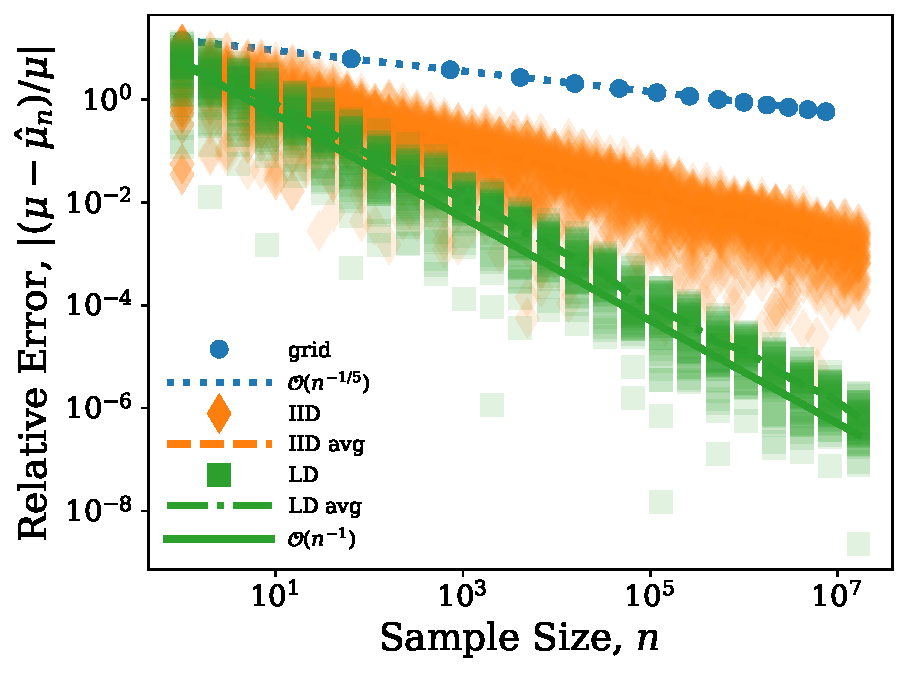
\includegraphics[width =10cm]{\figpath/n_is_16777216_d_is_6_n_rep_is_50_KeisterErrors.pdf}
	\caption{The relative error of approximating $\mu$ defined in \eqref{eq:keisterC} by the sample mean, $\hat{\mu}_n$ defined in \eqref{eq:sample_mean} for various choices of nodes, $\bsx_0, \bsx_1, \ldots$.  Grids have the largest error and LD nodes have the smallest error. \label{fig:keister-err}}
\end{figure}

Note the following from this example:
\begin{itemize}
	\item This integral is not particularly easy to evaluate numerically.  Even the best choice of nodes requires at least $n=100$ to get a relative error below $10\%$.

	\item \emph{Grid nodes.} Although grids may be attractive for low dimensional problems, e.g., $d = 1$, $2$, or $3$, they do poorly for this modest dimension, $d=6$.  Figure \ref{fig:grid} compares a $64$ point grid with $d = 2$ and $6$.  For $d = 6$, the possible sample sizes, $n$, are quite sparse, as shown in Figure \ref{fig:keister-err}.

	Choosing the nodes to lie on a grid corresponds to a tensor product midpoint cubature rule, which would normally be expected to have an error of $\mathcal{O}(n^{-2/d})$  for general $d$.  The error decay of $\mathcal{O}(n^{-1/5})$ rather than $\mathcal{O}(n^{-2/6})$ for this example may be due to the lack of smoothness of $f$ near the boundaries of the unit cube.

	\item \emph{IID nodes.}  Simple MC (orange) is a substantial improvement over grid nodes. As a reminder, for IID nodes the root mean squared error is
	\begin{equation}\label{eq:IIDerror}
		\sqrt{\mathbb{E}[(\mu - \hat{\mu})^2]} = \sqrt{\var(\hat{\mu})} = \sqrt{\frac{\var(f(\bsx))}{n}} = \frac{\mathrm{Std}(f(\bsx))}{n^{1/2}},
	\end{equation}
	where $\var$ denotes the variance and $\mathrm{Std}$ the standard deviation.  This $\mathcal{O}(n^{-1/2})$ decay is observed in Figure \ref{fig:keister-err}. For simple MC the sample size, $n$, can be any positive integer without affecting the rate of decay of the error.

	Whereas grid points collapse on top of one another when viewed in low dimensional projections, are IID points may be seen when viewed in any lower dimensional projection, as seen in Figure \ref{fig:iid}.  The disadvantage of IID points is that they form clusters and leave gaps.  This is because the position of any one node is independent of the position of the others.

	\item \emph{LD nodes.}  For qMC methods the error decays nearly like $\mathcal{O}(n^{-1})$, which for this example correponds to a reduction in error of several orders of magnitude compared to simple MC for large enough $n$.  Typically, LD sequences have preferred sample sizes.  For this Sobol' sequence, $n$ is chosen to be positive integer powers of $2$, which tends to give better accuracy than arbitrary $n$.

	Figure \ref{fig:ld} shows typical two-dimensional projections of a $64$ LD node set.  Visually, these nodes fill the unit cube better than IID nodes.  A quantitative measure of this, the discrepancy, is defined in Section \ref{sec:discrepancy}.  Constructions of LD node set are explained in the next section.

\end{itemize}

\begin{figure}
	\centering
	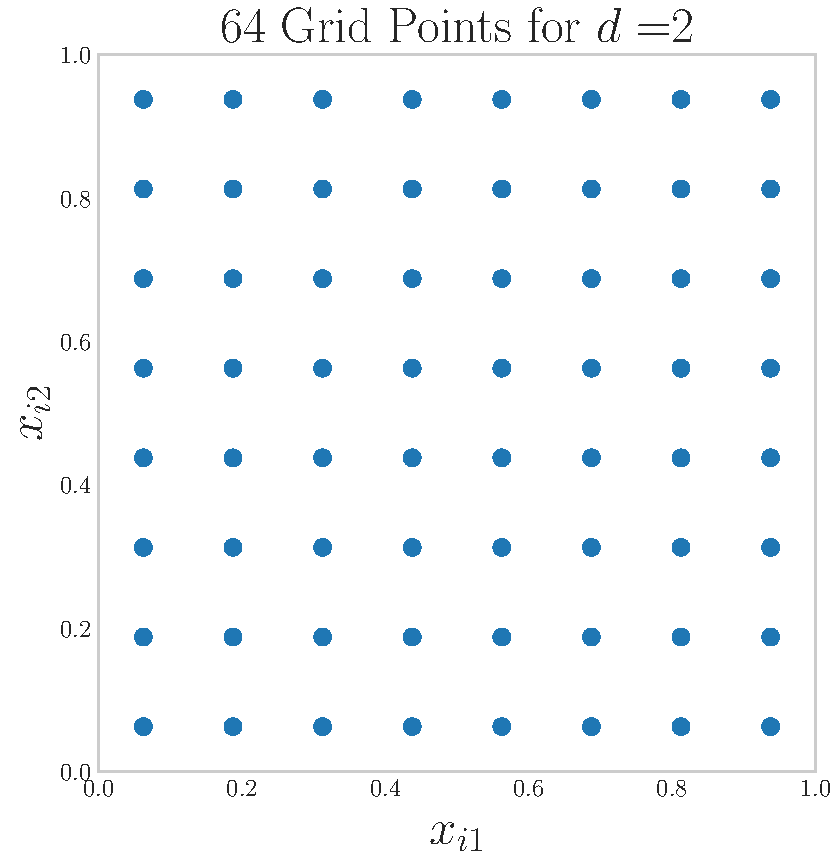
\includegraphics[width = 0.48\textwidth]{\figpath/64gridpts_d2.pdf}\quad
	%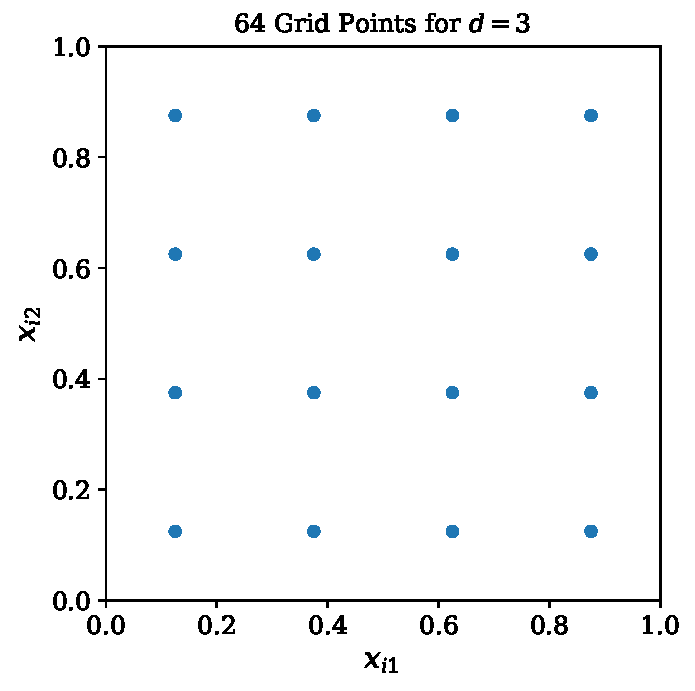
\includegraphics[width = 5cm]{\figpath/64gridpts_d3.pdf}\quad
	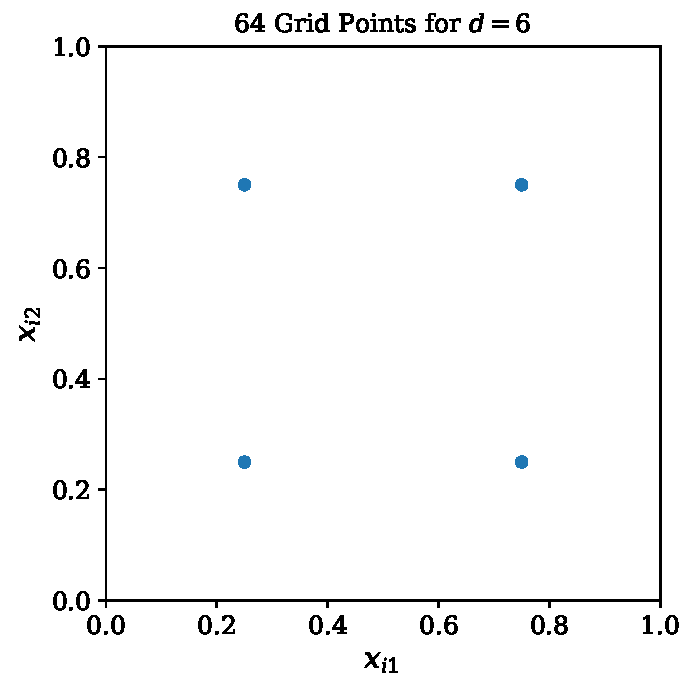
\includegraphics[width =  0.48\textwidth]{\figpath/64gridpts_d6.pdf}
	\caption{Although a two-dimensional grid covers the unit square rather well, a $d$-dimensional grid for modest $d$ does \emph{not} cover the unit cube well.  For example, one can only see four distinct points in a two dimensional projection of a six-dimensional grid with $64$ points. \label{fig:grid}}
\end{figure}

\begin{figure}
	\centering
	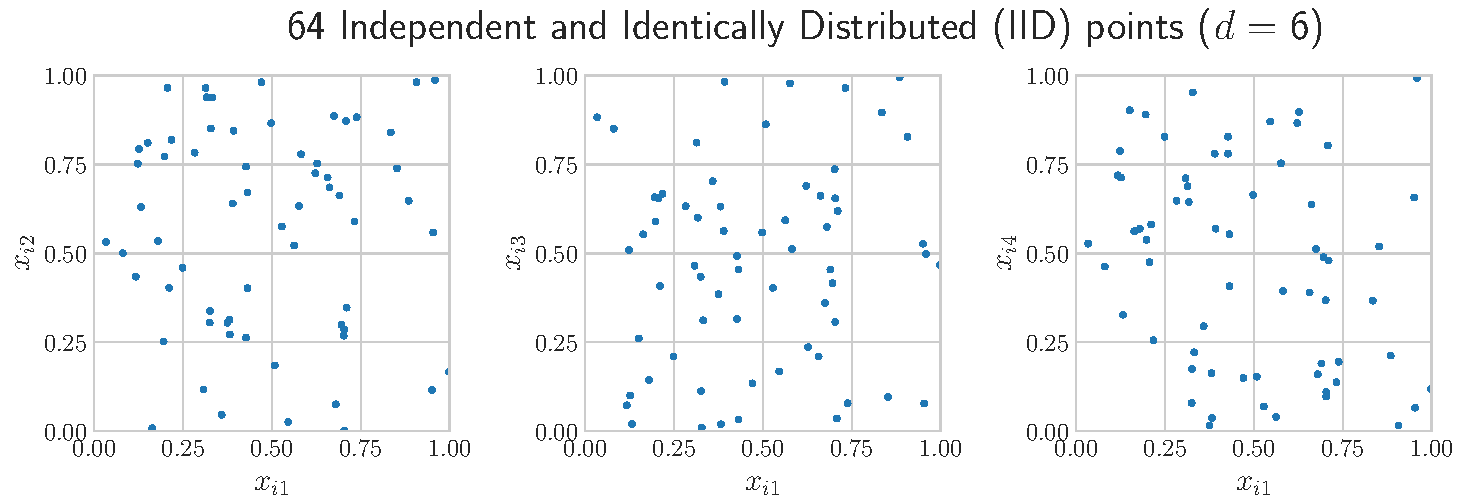
\includegraphics[width =\textwidth]{\figpath/64iidpts_d6.pdf}
	\caption{IID points cover the unit cube better than grid points, although one does observe clusters and gaps.  In any  projection there is  a similar looking distribution of all $64$ points \label{fig:iid}}
\end{figure}

\begin{figure}
	\centering
	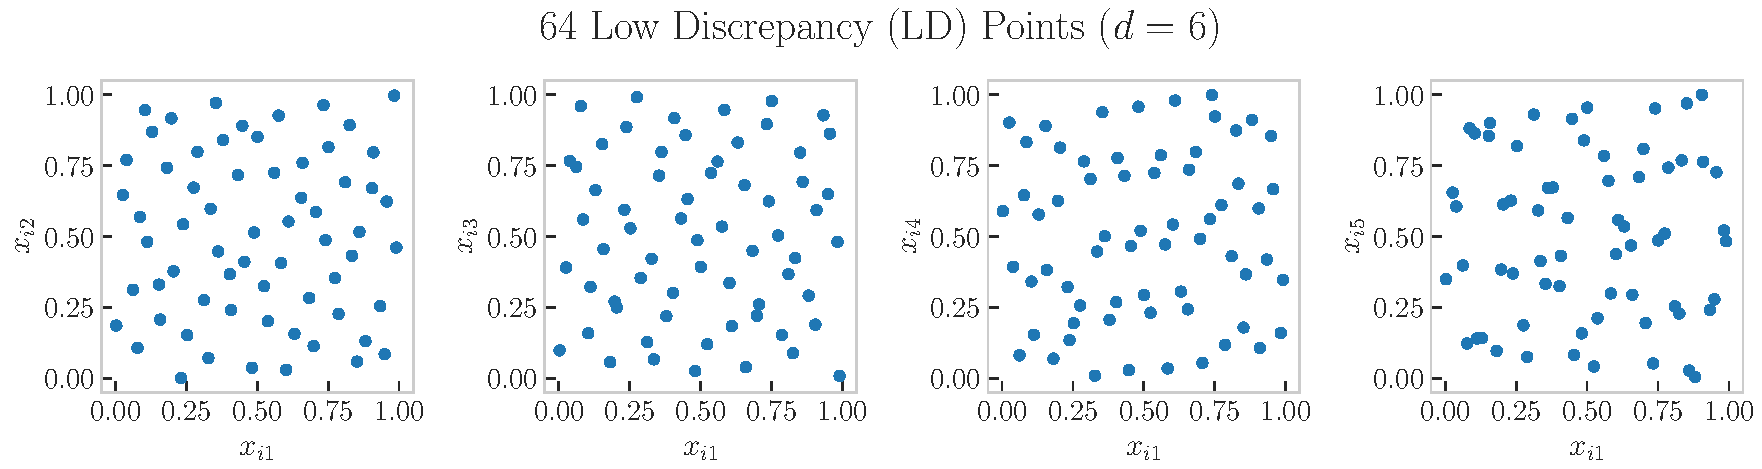
\includegraphics[width =\textwidth]{\figpath/64sobolpts_d6.pdf}
	\caption{LD points cover the unit cube better even better than IID points or grids.  In any  projection there is  a similar looking distribution of all $64$ points. \label{fig:ld}}
\end{figure}


\section{LD Sequence Constructions} \label{sec:construct}
This section introduces some of the most popular LD sequences.  What sets these apart from IID sequences is that the nodes are deliberately chosen and highly correlated to one another.

\subsection{Lattice Sequences} \label{sec:lattice}
The simplest LD construction is the family of good lattice points \cite{DicEtal22a,SloJoe94}.  As a finite node set, they are defined as follows:
\begin{equation} \label{eq:latticepts}
	\bsx_i = i\bsh/n \pmod \bsone, \qquad i = 0, \ldots, n-1,
\end{equation}
where $\bsh$ is a well chosen $d$-dimensional integer vector. Figure \ref{fig:latticeconstruct} illustrates this construction for $n = 16$ and $\bsh = (1,11)$.  Note that the set $\{\bsx_0, \ldots, \bsx_{n-1}\}$ defined in \eqref{eq:latticepts} is closed under addition modulo $\bsone$ so that it forms a group.


\begin{figure}
	\centering
	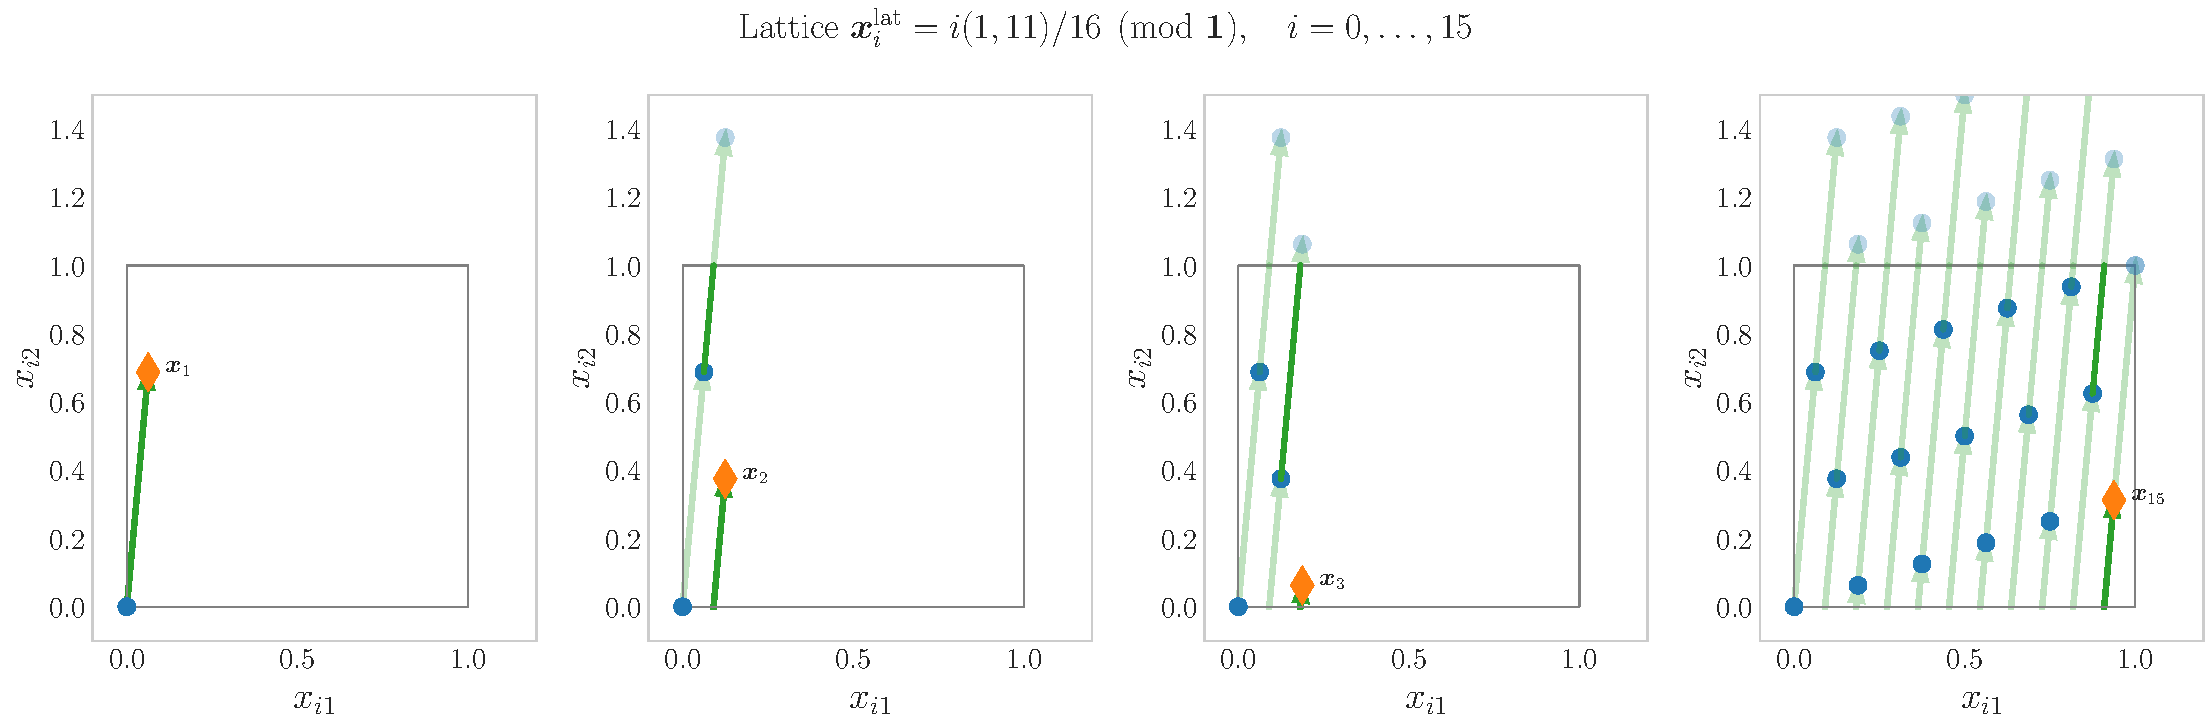
\includegraphics[width = \textwidth]{\figpath/16_lattice_construct_d2.pdf}
	\caption{The construction of a good lattice point set in two dimensions with $16$ nodes is obtained by moving $\bsh/n$ beyond the present point and wrapping around the boundaries of the square until one returns to the origin. \label{fig:latticeconstruct}}
\end{figure}


One disadvantage of this construction is that it is not readily extensible. For the example in Figure \ref{fig:latticeconstruct} the first $8$ points do not fill the unit square.  However, the set of points defined by even $i$ do a reasonable job.  This suggests a method for defining lattice sequences that was proposed independently by \cite{Mai81a} and \cite{HicEtal00}.

Let's start with the one-dimensional extensible lattice that is defined by the van der Corput sequence, $\{\phi_b(0), \phi_b(1), \ldots\}$.  This involves reflecting the digits of the integer $i$ in base $b$ about the decimal point.  For example, $i = 6 = 110_{2}$ gives $\phi_2(6) = {}_20.011 = 3/8$, or in general,
\begin{equation} \label{eq:vdc}
	\phi_b(i) := i_0 b^{-1} + i_1 b^{-2} + i_2 b^{-3} + \cdots \in [0,1) \quad \text{for }
		i = i_0 + i_1b + i_2 b^2 + \cdots .
\end{equation}
For all non-negative integers, $m$, the first $n = b^m$ nodes in the van der Corput sequence correspond to the evenly spaced nodes $\{0, b^{-m}, \ldots, 1 - b^{-m} \}$---albeit in a different order.

To construct an extensible lattice, we replace $i/n$ in \eqref{eq:latticepts} by $\phi_b(i)$ to get
\begin{equation} \label{eq:extensiblelattice}
	\bsx_i =\phi_b( i)\bsh \pmod \bsone, \qquad i = 0, 1 , \ldots.
\end{equation}
This reordering of points from the original construction allows us to preserve the lattice structure for the first $b^m$ points for any non-negative integer $m$. That is, $\{\bsx_0, \ldots, \bsx_{2^m-1}\}$ is a closed under addition modulo $\bsone$.

Figure \ref{fig:extensiblelatticeconstruct} shows the first $4$, $8$, and $16$ points of the earlier example in Figure \ref{fig:latticeconstruct}.  The blue nodes are a copy of the nodes in the plot to the left, and the the orange nodes correspond to a shifted copy of the blue nodes modulo $\bsone$.  For the left plot, the shift is $\phi_2(2)\bsh = (1,11)/4$ or equivalently $(0.25,0.75)$.  For the middle plot, the shift is $\phi_2(4)\bsh = (1,11)/8$ or equivalently $(0.125,0.375)$. For the right plot, the shift is $\phi_2(8)\bsh = (1,11)/16$  or equivalently $(0.0625,0.6875)$.

\begin{figure}
	\centering
	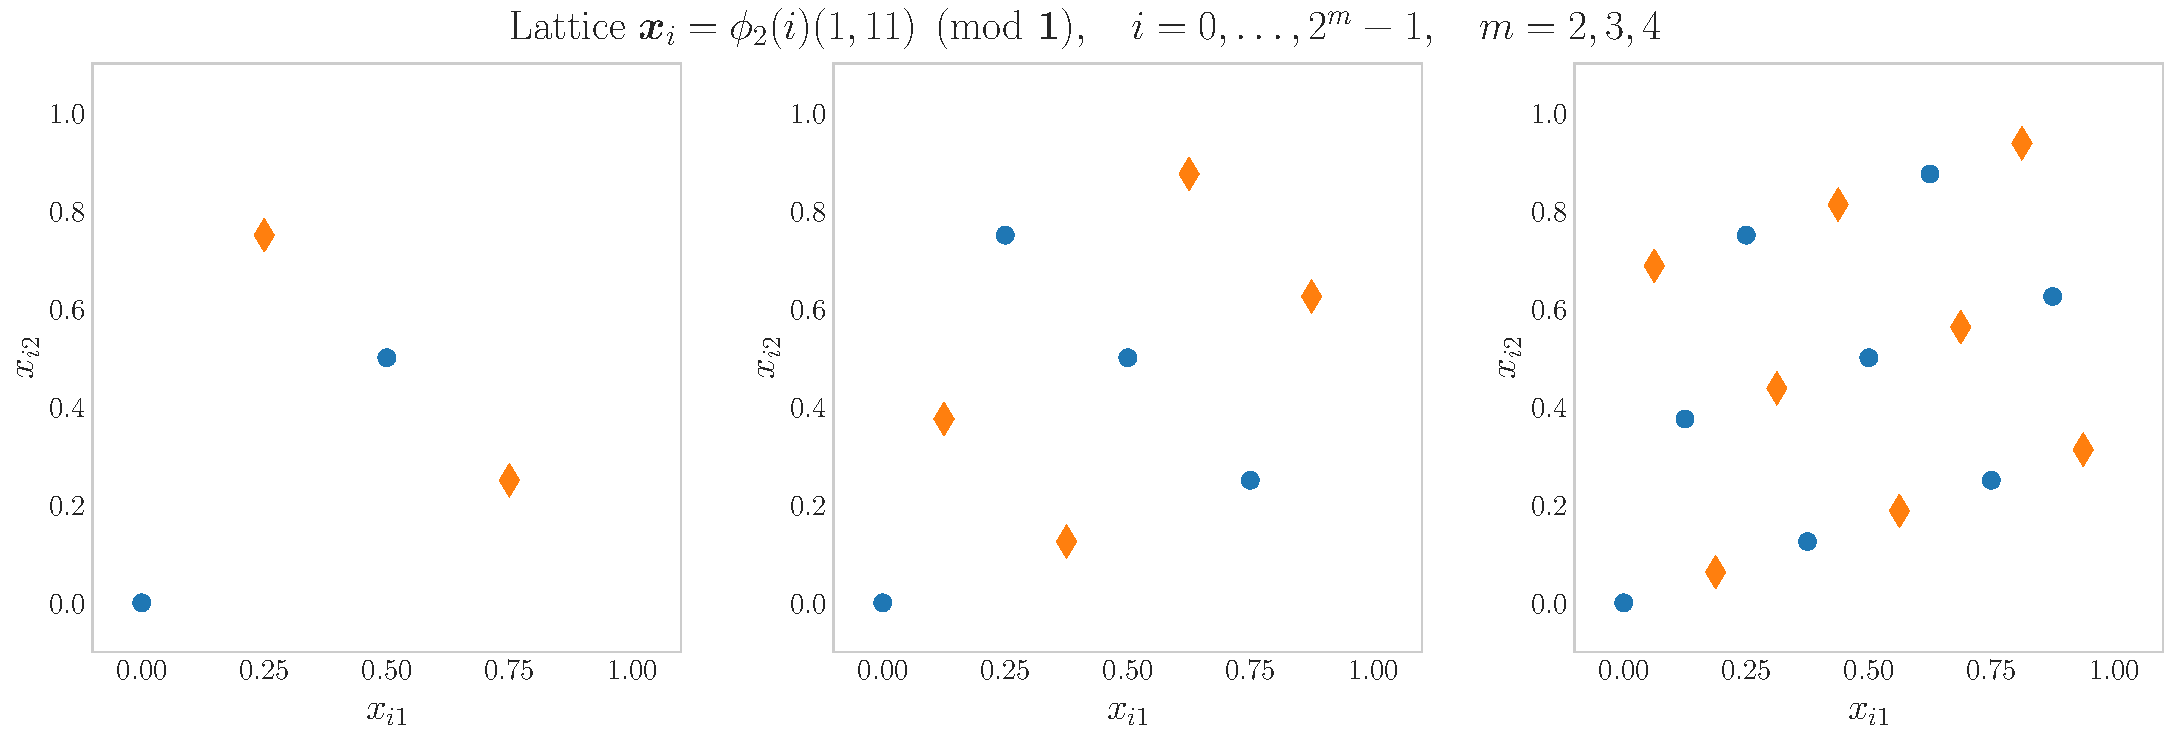
\includegraphics[width = \textwidth]{\figpath/16_extensible_lattice_construct_d2.pdf}
	\caption{An extensible lattice corresponding to  Figure \ref{fig:latticeconstruct}  with the nodes reordered using the van der Corput sequence in base $2$.  For each plot the blue nodes are a copy of the nodes to the left and the orange nodes are a shifted copy (modulo $\bsone$) of the blue nodes. \label{fig:extensiblelatticeconstruct}}
\end{figure}

For the example in Figure \ref{fig:extensiblelatticeconstruct}, increasing $n$ beyond $16$ repeats the orginal points because the generating vector $\bsh$ has integers less than $16$.  Obtaining a truly extensible lattice sequence requires that $\bsh$ be a vector of generalized integers---essentially integers with infinite numbers of nonzero digits---as explained in \cite{HicNie03a}, where the existence of good generating vectors is also proved.  In practice, one searches computationally for a $\bsh$ that produces good set of lattice nodes of size $n = b^m$ for a range of $m$ \cite{HicEtal00}.

\subsection{Digital Sequences} \label{sec:digital}

Another family of LD sequences that also builds from the van der Corput sequence of \eqref{eq:vdc} is digital sequences \cite{DicPil10a,Nie92}.  For simplicity, we restrict ourselves to $b = 2$ and let $\oplus$ denote digitwise addition, e.g., $3/8 \oplus 3/4 = {}_20.011 \oplus {}_20.110 = {}_20.101 = 5/8$.  A digital sequence is defined as
\begin{equation} \label{eq:digital}
	\bsx_i := i_0 \bsc_1 \oplus i_1 \bsc_2 \oplus i_2 \bsc_3 \oplus \cdots \in [0,1)^d \quad \text{for }
	i = i_0 + i_12 + i_2 2^2 + \cdots,
\end{equation}
where $\bsc_1, \bsc_2, \ldots$ are carefully chosen.  If $c_{ij\ell}$ denotes the $\ell^{\text{th}}$ digit of the $j^{\text{th}}$ coordinate of $\bsc_i$, then in the literature one may see the generators of digital sequences stored as generating matrices, $\mathsf{C}_j = (c_{ij\ell})_{\ell,i = 1}^{M,N}$ for $j = 1, \ldots, d$, where $M$ is th maximum number of bits in the expression for $\bsx_i$, say $52$, and $2^N$ is the maximum number of nodes that is intended to be generated.

Digital sequence generators can be found via number theory or numerical search.  The



\section{Discrepancy} \label{sec:discrepancy}
\section{Randomization} \label{sec:random}
\section{Stopping Criteria} \label{sec:stop}
\section{Reformulating Our Problem} \label{sec:reformulate}
\section{Ongoing Research} \label{sec:onging}
\section{Conclusion} \label{sec:conclusion}



\bibliographystyle{spmpsci}
\bibliography{FJH23,FJHown23}


\end{document}

